\section{Design Details for Evolution Scenarios}
%TODO "describes the adaptive evolution scenari of.." changed to "changes in "
In this chapter we provide the detailed design documentation for each of the evolution scenarios
introduced in the prior section. Sec. \ref{App} sketches the design decision for the Mobile App that provides a second sales channel next to the existing Pick-up Shop. Sec. \ref{Docker} describes the adaptive cahnges of setting up a Docker environment to simplify the update process. They are both based on, or at least use the Hybrid Cloud-based Variant of CoCoME \cite{SWB-469002735}. In contrast, Sec. \ref{MS} provides a detailed design documentation of a new architectural version of CoCoME. This perfective evolution scenario is realized based on the Microservice idea.

\subsection{Design Decisions for the Mobile App} \label{App}
	%TODO Add most important information od App-Paper


\subsection{Setting up a Docker environment} \label{Docker}
	%TODO Add most important information of docker paper
	Looking to the changes for the Docker project, you can see in figure \ref*{techStack} the changes are affecting the technology stack by adding additional layers. More detailed, the given CoCoME Stack is moved into the Docker Deamon, which runs a Linux distribution. As mentioned, the original parts of the stack, like Glassfish and the Java Virtual Machine, are still a part of the stack.\\
	\begin{figure}[H]
		\centering
		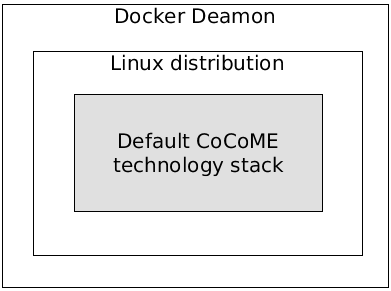
\includegraphics[width = 0.5\textwidth]{img/tech_stack_CoCoME.png}
		\caption{Extended technology stack CoCoME}
		\label{techStack}
	\end{figure}
	
	The Dockerfile defines an environment based on the latest version of Ubuntu 16:04. Onto it there is installed Maven, Git and Java by using the Ubuntu package manager.\\
	Git has two purposes: On the one hand it is used to download the most recent version of CoCoME.	On the other hand, it is used to download a prefabricated version of Glassfish that already includes domains and other adjustments required for CoCoME. Java is required by Glassfish and CoCoME as they need the Java Virtual Machine. Maven is needed to deploy the latest version of CoCoME onto the provided Glassfish servers.
	
	
	\subsubsection{Deployment}\hfil \\
	During the development, it was decided to implement and to provide two different versions. The first version always pulls the most recent CoCoME source code from GitHub, downloads the entire dependencies with maven, compiles and builds the project and finally, deploys CoCoME on the Glassfish servers. . As a consequence. creating and starting a Docker Container takes about one hour.\\
	In contrast, the second version only  pulls a prefabricated version of CoCoME from GitHub. Therefore, pulling the source code up to building the project is skipped. As a consequence, Maven does not have to be included in the technology stack. Solely, deploying CoCoME on the glassfish server is necessary.\\
	This reduces the deployment time to a few minutes but has a disadvantage: The prefabricated version is updated manually. Therefore, it is sometime not the most recent version.\\
	By providing both, a fast deploying version and a current version, the user can choose whats the best for its situation.
	
	\begin{figure}[h]
		\centering
		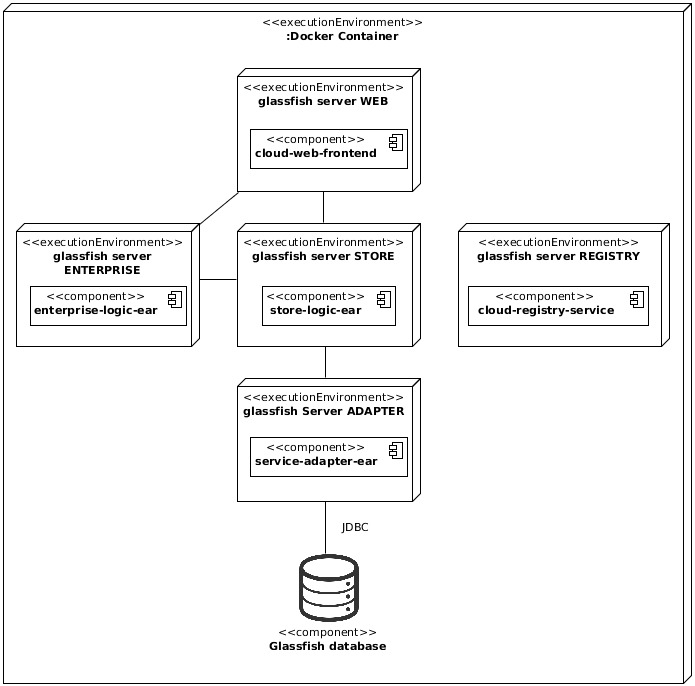
\includegraphics[width = 0.9\textwidth]{img/docker_Container_Deployment.png}
		\caption{Deployment diagram CoCoME}
		\label{Deploym_CoCoME}
	\end{figure}
	
	As shown above in figure \ref*{Deploym_CoCoME} the docker Container contains five different Glassfish servers. In particular they are called \textit{WEB}, \textit{ENTERPRISE}, \textit{STORE}, \textit{REGISTRY} and \textit{ADAPTER} and correspond to the given by the CoCoME deplyoment setup. By default, Glassfish provides a Derby DB that is connected to the server Adapter using Java Database Conectivity (JDBS) interface.\\
	As mentioned before, CoCoME is deployed inside the docker container on the same way it is usually deployed. This means the maven generated archive files \textit{cloud-web-frontend},\textit{enterprise-logic-ear},\textit{store-logic-ear}\textit{cloud-registry-sevice} and \textit{service-adapter-ear} are deployed to the servers with the following assignment:
	\begin{figure}[H]
		\centering
		\begin{tabular}{p{0.25\textwidth}|p{0.01\textwidth}p{0.25\textwidth}}
			Server && Deployment file \\
			\hline
			WEB && cloud-web-frontend  \\
			ENTERPRISE && enterprise-logic-ear  \\
			STORE && store-logic-ear  \\
			REGISTRY && cloud-registry-service  \\
			ADAPTER && service-adapter-ear \\	
		\end{tabular}
		\caption{Assignment of archive files to Servers}
		\label{table_assignment}
	\end{figure}
	\ref{table_assignment} demonstrates the assignment between the archive files and the servers as it is implemented and also recommended by the CoCoME deployment guide. This information is also represented in Fig. 2. As mentioned earlier, there are two versions of this Docker project. Both deploy the CoCoME main program with this assignment.\\ \\
	
	In addition, the fast version can be extends by the pickup shop\footnote{\url{https://github.com/cocome-community-case-study/cocome-cloud-jee-web-shop}}. This pickup-shop runs inside a separate container which is shown in figure \ref{Deploym_Pickup}.  
	\begin{figure}[h]
		\centering
		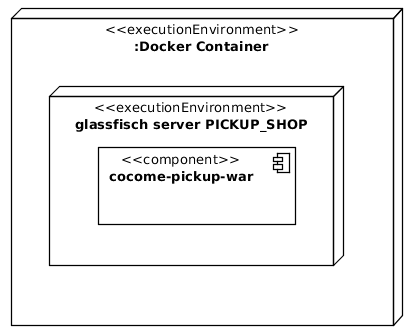
\includegraphics[width = 0.4\textwidth]{img/docker_Container_PickUP.png}
		\caption{Deployment diagram CoCoME Pickup Shop}
		\label{Deploym_Pickup}
	\end{figure}
	As shown in figure \ref*{Deploym_Pickup}, this container provides only one Glassfish server.
	\begin{figure}[H]
		\centering
		\begin{tabular}{p{0.25\textwidth}|p{0.01\textwidth}p{0.25\textwidth}}
			Server && Deployment file \\
			\hline
			PICKUP\_SHOP && cocome-pickup-war \\	
		\end{tabular}
		\caption{Assignment archive files to Servers}
		\label{table_assignment_pickup}
	\end{figure}
	To control the start of both containers, precisely the CoCoME and the Pick Up Shop, another specific file is needed: the Docker Compose file. It ensures that the CoCoME Container is active, before the pickup-shop container is starting. This is necessary as the Pickup Shop requires a running instance of CoCoME to register itself.\\
	Also CoCoME runs without the pickup-shop, the pickup-shop does not work without an running instance of CoCoME.\\
	Both containers need to communicate with each other. By default, docker prohibits any outgoing and ingoing communication from an in a container. This is solved by opening specific ports through which the communication is possible. Which ports the containers can use is specified in the Docker Compose file as well.
	
\subsection{Using Microservices Technology} \label{MS}
	\begin{itemize}
		\item je microservice absatz mit entsprechenden Sequenzendiagram %fertig machen der implementierung
		\item frontend? muss dazu auch das gemacht werden?
		\item ein blocktext zu mehereren diagrammen oder diagramme zwischen text?
		
	
			\item je die einzelnen module und szenarien erlaeutern in dem diese sinnvoll sind
	\end{itemize}
	
		\subsubsection{Products}
		abstrahieren der Produktinformationen 
		
		\subsubsection{Stores}
		einzelne Laeden alleinstehend abbilden um nach bedarf neue microservices alias laeden starten zu können
		
		\subsubsection{Enterprise}
		aehnlich zu stroes
		
		\subsubsection{Reports}
		stellt alleinigen aufgaben bereich dar, entsprechen undabhaengig darzustellen von anderem.




	
	
(grafik/Tabelle  -> oben oder unten caption)